% =============================================================================
%  IEEE 39-bus New England test system – finalized layout
%  Changes:
%   (1) B03 moved to y=8.0. B04 and B14 placed consecutively to the right at y=8.0.
%   (2) Added a fully structured "DS_2" cluster centrally for B04, B14, and B06.
%   (3) Routing mathematically updated to ensure ZERO overlap with new DS2 layout.
%   (4) ALL lines leave busbars strictly vertically (V-H-V routing or U-shapes).
%   (5) Taps are offset to ensure NO line leaves from the exact edges.
%   (6) Added organic, light grey background shapes around all DS areas.
% =============================================================================

\documentclass[tikz,border=10pt]{standalone}
\usepackage{circuitikz}
\usepackage{amsmath}
\usepackage{xcolor}
\usetikzlibrary{positioning,fit,backgrounds,arrows.meta,shapes.geometric,%
	shapes.symbols,calc,decorations.pathmorphing}

% TU Darmstadt palette
\definecolor{tudaBlue}{HTML}{004E8A}
\definecolor{tudaYellowGreen}{HTML}{B1BD00}
\definecolor{tudaTeal}{HTML}{CC4C03}
\definecolor{wpfill}{HTML}{E0F0D8}
\definecolor{dsfill}{HTML}{E5E4E2}

% Pics
\tikzset{
	pics/windpark/.style={code={
			\draw[line width=0.7pt] (-0.05,0) rectangle (0.05,0.60);
			\draw[line width=0.6pt] (0,0.60) circle (0.07);
			\foreach \a in {90+20,210+20,330+20}{%
				\draw[line width=0.55pt]
				(0,0.60) -- ++(\a+4:0.34) -- ++(\a-8:-0.04) -- cycle;}
	}},
	pics/trafo2w/.style={code={
			\draw[line width=0.85pt] (0, 0.14) circle (0.23);
			\draw[line width=0.85pt] (0,-0.14) circle (0.23);
	}},
	pics/trafo3w/.style={code={
			\draw[line width=0.85pt] (0, 0.18) circle (0.23);
			\draw[line width=0.85pt] (-0.17,-0.10) circle (0.23);
			\draw[line width=0.85pt] ( 0.17,-0.10) circle (0.23);
	}},
}

% Styles
\tikzset{
	bus/.style         ={line cap=rect, line width=1.9pt, black},
	tline/.style       ={line width=0.6pt, black},
	trafoln/.style     ={line width=0.6pt, black},
	couplerln/.style   ={line width=0.6pt, black, dashed, dash pattern=on 2.2pt off 1.7pt},
	zoneline/.style    ={line width=1.3pt, black!70, loosely dotted},
	loadarrow/.style   ={-{Latex[length=2.4mm,width=1.8mm]}, black, line width=0.75pt},
	gencircle/.style   ={circle, draw, line width=0.7pt, fill=none, minimum size=7mm, inner sep=0pt, font=\small},
	slackcircle/.style ={circle, draw, line width=0.9pt, fill=none, minimum size=7mm, inner sep=0pt, font=\small},
	wpcircle/.style    ={circle, draw, line width=0.7pt, fill=none, minimum size=7mm, inner sep=0pt, font=\small},
	dsobox/.style      ={rectangle, draw, line width=1pt, rounded corners=1.5pt, fill=dsfill, minimum width=0.75cm, minimum height=0.42cm, inner sep=1pt, font=\scriptsize, align=center},
	buslabel/.style    ={font=\scriptsize\color{black}, inner sep=1pt},
	zonelbl/.style     ={font=\Large\bfseries\color{black}},
	dslbl/.style 	   ={font=\large\bfseries\color{black}},
	genlbl/.style      ={font=\footnotesize, inner sep=1pt},
	wplbl/.style       ={font=\footnotesize, inner sep=1pt},
}

\newcommand{\vhvo}[5]{ \draw[tline] let \p1=($(#1)+(#2,0)$), \p2=($(#3)+(#4,0)$) in (\p1) -- (\x1,#5) -- (\x2,#5) -- (\p2); }

\def\tTop{0.37} \def\tBot{0.37} \def\tThvTop{0.41} \def\tThvBot{0.33}

\begin{document}
	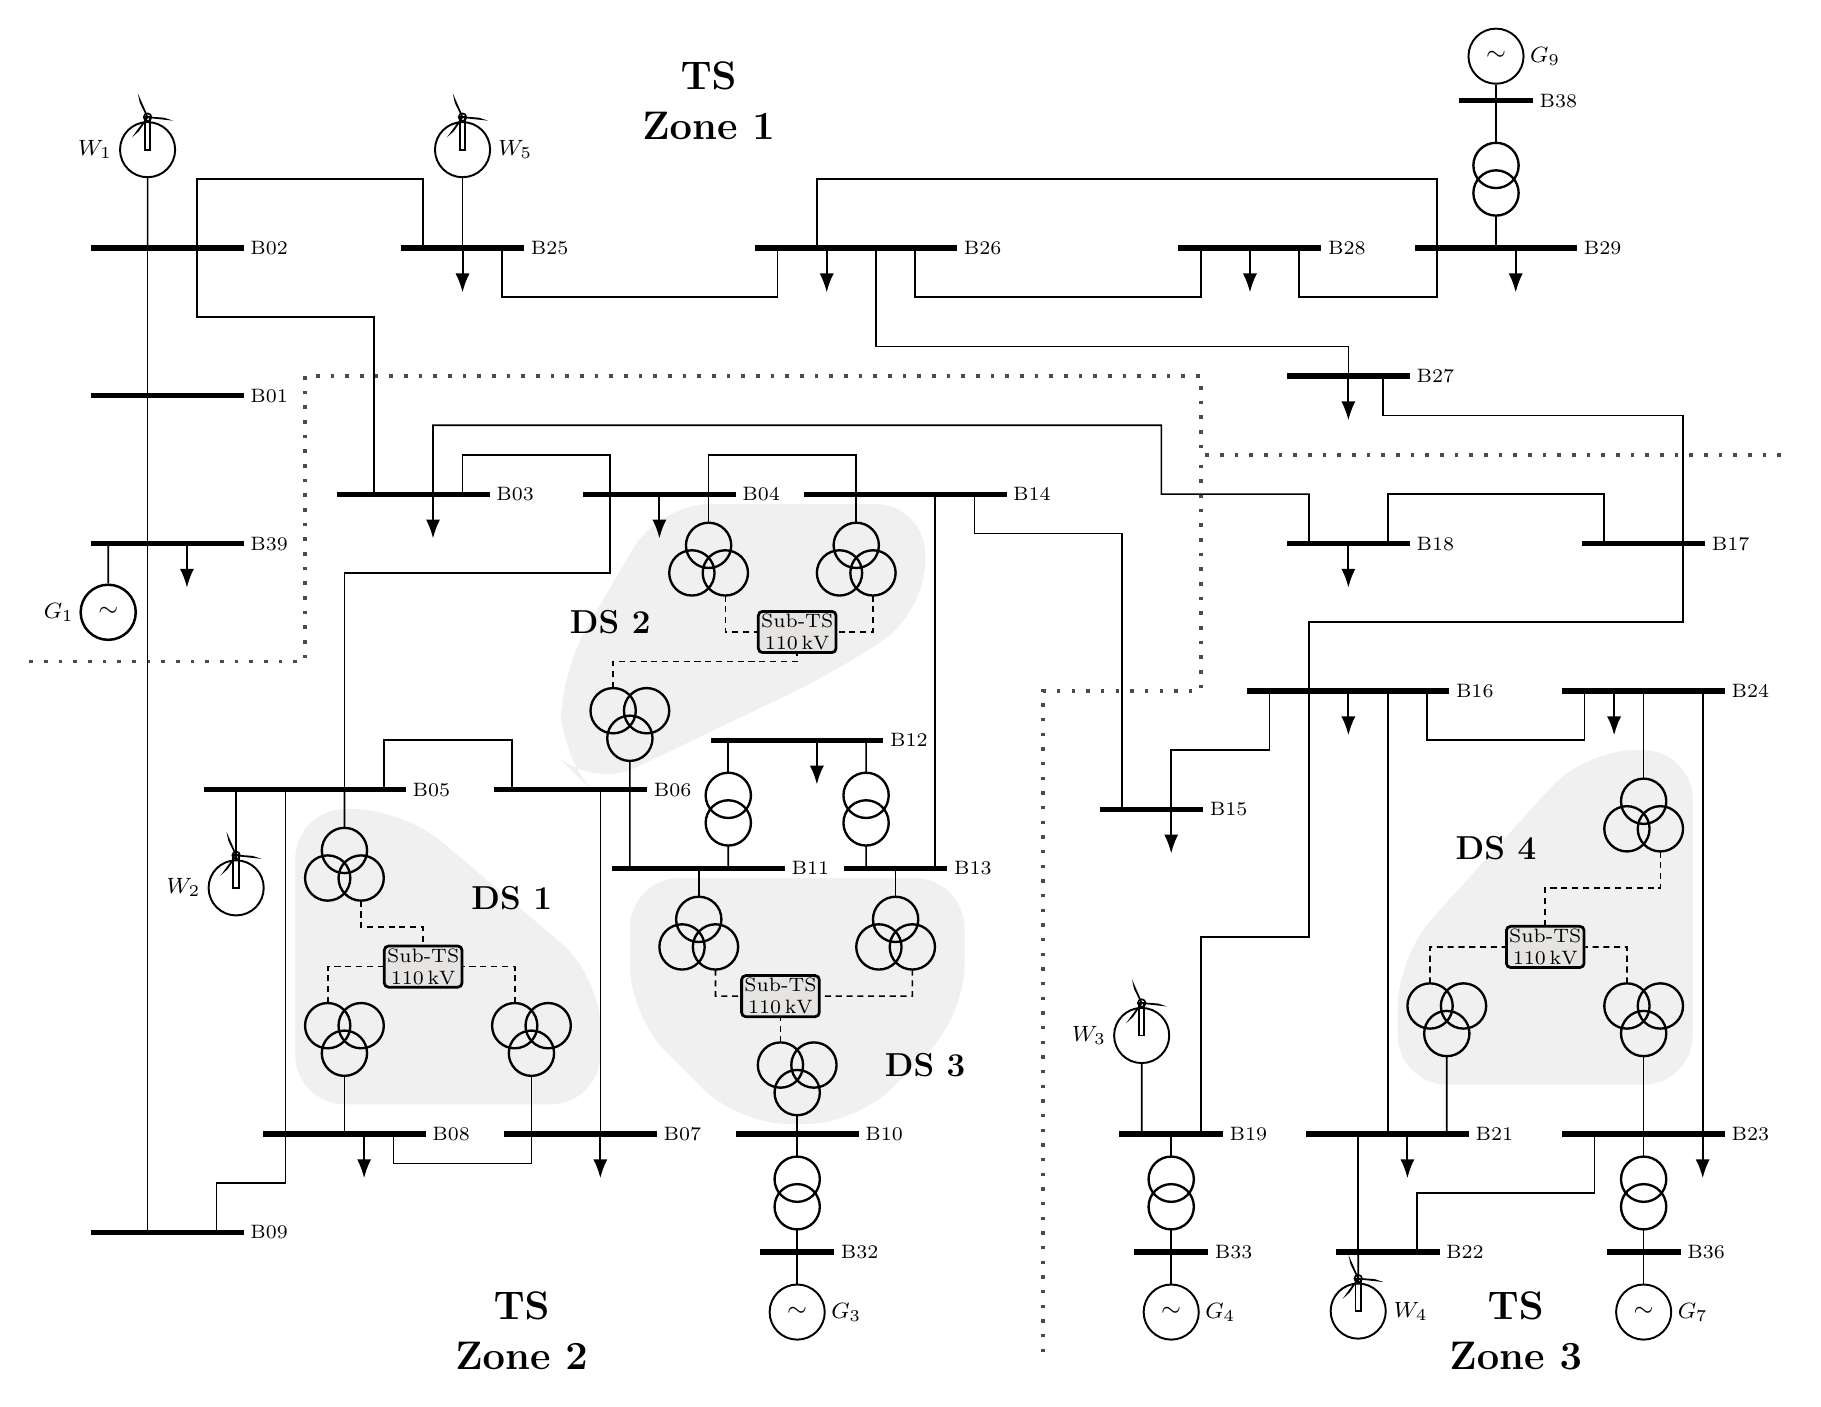
\begin{tikzpicture}[x=1.25cm, y=1.25cm]
		
		% =============================================================================
		%  1.  Bus coordinate map
		% =============================================================================
		% ---- Zone 1 ----
		\coordinate (B02) at ( 1.0, 10.5);
		\coordinate (B01) at ( 1.0,  9.0);
		\coordinate (B39) at ( 1.0,  7.5);
		\coordinate (B25) at ( 4.0, 10.5);
		\coordinate (B26) at ( 8.0, 10.5);
		\coordinate (B27) at (13.0,  9.2);
		\coordinate (B28) at (12.0, 10.5);
		\coordinate (B29) at (14.5, 10.5);
		\coordinate (B38) at (14.5, 12.0);
		
		% ---- Zone 2 ----
		\coordinate (B03) at ( 3.5,  8.0);
		\coordinate (B04) at ( 6.0,  8.0);
		\coordinate (B14) at ( 8.5,  8.0);
		\coordinate (B05) at ( 2.4,  5.0);
		\coordinate (B06) at ( 5.1,  5.0);
		\coordinate (B07) at ( 5.2,  1.5);
		\coordinate (B08) at ( 2.8,  1.5);
		\coordinate (B09) at ( 1.0,  0.5);
		\coordinate (B12) at ( 7.4,  5.5);
		\coordinate (B11) at ( 6.4,  4.2);
		\coordinate (B13) at ( 8.4,  4.2);
		\coordinate (B10) at ( 7.4,  1.5);
		\coordinate (B32) at ( 7.4,  0.3);
		
		% ---- Zone 3 ----
		\coordinate (B15) at (11.0,  4.8);
		\coordinate (B16) at (13.0,  6.0); 
		\coordinate (B17) at (16.0,  7.5); 
		\coordinate (B18) at (13.0,  7.5);
		\coordinate (B19) at (11.2,  1.5);
		\coordinate (B21) at (13.4,  1.5);
		\coordinate (B22) at (13.4,  0.3);
		\coordinate (B23) at (16.0,  1.5); 
		\coordinate (B24) at (16.0,  6.0); 
		\coordinate (B33) at (11.2,  0.3);
		\coordinate (B36) at (16.0,  0.3);
		
		% =============================================================================
		%  2.  Zone separators (dashed lines)
		% =============================================================================
		\draw[zoneline]
		(-0.4, 6.3) -- (2.4, 6.3) -- (2.4, 9.2) -- (11.5, 9.2)
		-- (11.5, 8.4) -- (17.5, 8.4);
		
		\draw[zoneline]
		(11.5, 8.3) -- (11.5, 6.0) -- (9.9, 6.0) -- (9.9, -0.8);
		
		% =============================================================================
		%  3.  Bus bars + labels
		% =============================================================================
		\newcommand{\drawbuslbl}[3][0.45]{%
			\draw[bus] ($(#2)+(-#1,0)$) -- ($(#2)+(#1,0)$);
			\node[buslabel,anchor=west] at ($(#2)+(#1+0.06,0)$) {#3};
		}
		
		\drawbuslbl[0.75]{B39}{B39}
		\drawbuslbl[0.75]{B01}{B01}
		\drawbuslbl[0.75]{B02}{B02}
		\drawbuslbl[0.6]{B25}{B25}
		\drawbuslbl[1.0]{B26}{B26}
		\drawbuslbl[0.6]{B27}{B27} 
		\drawbuslbl[0.7]{B28}{B28}
		\drawbuslbl[0.8]{B29}{B29}
		
		\drawbuslbl[0.75]{B03}{B03}
		\drawbuslbl[0.75]{B04}{B04}
		\drawbuslbl[1.0]{B14}{B14}
		\drawbuslbl[1.0]{B05}{B05} 
		\drawbuslbl[0.75]{B06}{B06} 
		\drawbuslbl[0.75]{B07}{B07}
		\drawbuslbl[0.8]{B08}{B08}
		\drawbuslbl[0.75]{B09}{B09}
		\drawbuslbl[0.85]{B12}{B12}
		\drawbuslbl[0.85]{B11}{B11}
		\drawbuslbl[0.5]{B13}{B13}
		\drawbuslbl[0.6]{B10}{B10}
		
		\drawbuslbl[0.6]{B18}{B18}
		\drawbuslbl[0.6]{B17}{B17} 
		\drawbuslbl[0.5]{B15}{B15}
		\drawbuslbl[1.0]{B16}{B16}
		\drawbuslbl[0.8]{B24}{B24}
		\drawbuslbl[0.5]{B19}{B19}
		\drawbuslbl[0.8]{B21}{B21} 
		\drawbuslbl[0.5]{B22}{B22}
		\drawbuslbl[0.8]{B23}{B23}
		
		\drawbuslbl[0.35]{B32}{B32}
		\drawbuslbl[0.35]{B33}{B33}
		\drawbuslbl[0.35]{B36}{B36}
		\drawbuslbl[0.35]{B38}{B38}
		
		% =============================================================================
		%  4.  Transmission lines (Strictly V-H-V, none leave from the exact edges)
		% =============================================================================
		% ---- Zone 1 ----
		\draw[tline] ($(B02)+(-0.2,0)$) -- ($(B01)+(-0.2,0)$);
		\draw[tline] ($(B01)+(-0.2,0)$) -- ($(B39)+(-0.2,0)$); 
		\vhvo{B39}{-0.2}{B09}{-0.2}{4.0}
		\vhvo{B02}{ 0.3}{B25}{-0.4}{11.2}
		\vhvo{B25}{ 0.4}{B26}{-0.8}{10.0}
		\vhvo{B26}{ 0.2}{B27}{ 0.0}{9.5}
		\vhvo{B26}{ 0.6}{B28}{-0.5}{10.0}
		\vhvo{B28}{ 0.5}{B29}{-0.6}{10.0}
		\vhvo{B26}{-0.4}{B29}{-0.6}{11.2}
		
		% ---- Zone 2 ----
		\vhvo{B02}{ 0.3}{B03}{-0.4}{9.8}
		\vhvo{B03}{0.5}{B04}{-0.5}{8.4}
		\vhvo{B04}{0.5}{B14}{-0.5}{8.4}
		\vhvo{B04}{-0.5}{B05}{ 0.4}{7.2} 
		\draw[tline] ($(B05)+(-0.2,0)$) -- ($(B08)+(-0.6,0)$);
		\vhvo{B05}{ 0.8}{B06}{-0.6}{5.5}
		\vhvo{B06}{ 0.3}{B07}{ 0.2}{3.0}
		\vhvo{B07}{-0.5}{B08}{ 0.5}{1.2}
		\vhvo{B08}{-0.6}{B09}{ 0.5}{1.0}
		\draw[tline] ($(B03)+(0.2,0)$) -- ($(B03)+(0.2,0.7)$) -- ($(B03)+(7.6,0.7)$) -- ($(B03)+(7.6,-0.0)$) -- ($(B18)+(-0.4,0.5)$) -- ($(B18)+(-0.4,0.0)$);
		\draw[tline] ($(B06)+(0.6,0)$) -- ($(B11)+(-0.7,0)$);
		\vhvo{B14}{ 0.3}{B13}{ 0.4}{6.2} 
		
		% ---- Zone 3 ----
		\vhvo{B14}{ 0.7}{B15}{-0.3}{7.6}
		\vhvo{B17}{ 0.4}{B27}{0.35}{8.8}
		\vhvo{B17}{-0.4}{B18}{ 0.4}{8.0}
		\vhvo{B17}{ 0.4}{B16}{-0.4}{6.7}
		\vhvo{B15}{ 0.2}{B16}{-0.8}{5.4}
		\vhvo{B16}{-0.4}{B19}{ 0.3}{3.5}
		\vhvo{B16}{ 0.4}{B21}{ 0.0}{3.0}
		\vhvo{B16}{ 0.8}{B24}{-0.6}{5.5}
		\draw[tline] ($(B21)+(-0.3,0)$) -- ($(B22)+(-0.3,0)$);
		\vhvo{B22}{ 0.3}{B23}{-0.5}{0.9}
		\vhvo{B24}{ 0.6}{B23}{ 0.6}{3.5}
		
		% =============================================================================
		%  5.  Network 2W OLTCs at B12 
		% =============================================================================
		\coordinate (Tr1112) at (6.7, 4.8);
		\draw[trafoln] ($(B12)+(-0.7,0)$) -- ($(Tr1112)+(0,\tTop)$);
		\pic at (Tr1112) {trafo2w};
		\draw[trafoln] ($(Tr1112)+(0,-\tBot)$) -- ($(B11)+(0.3,0)$);
		
		\coordinate (Tr1213) at (8.1, 4.8);
		\draw[trafoln] ($(B12)+(0.7,0)$) -- ($(Tr1213)+(0,\tTop)$);
		\pic at (Tr1213) {trafo2w};
		\draw[trafoln] ($(Tr1213)+(0,-\tBot)$) -- ($(B13)+(-0.3,0)$);
		
		% =============================================================================
		%  6.  Machine step-up transformers + synchronous machines
		% =============================================================================
		\node[slackcircle] (G1) at (0.4, 6.8) {$\sim$};
		\draw[trafoln] ($(B39)+(-0.6,0)$) -- (G1);
		\node[genlbl,left=0.03cm of G1] {$G_1$};
		
		\coordinate (TrG3) at (7.4, 0.9);
		\draw[trafoln] ($(B10)+(0.0,0)$) -- ($(TrG3)+(0,\tTop)$);
		\pic at (TrG3) {trafo2w};
		\draw[trafoln] ($(TrG3)+(0,-\tBot)$) -- (B32);
		\node[gencircle,below=0.40cm of B32] (G3) {$\sim$};
		\draw[trafoln] (B32) -- (G3);
		\node[genlbl,right=0.03cm of G3] {$G_3$};
		
		\coordinate (TrG4) at (11.2, 0.9);
		\draw[trafoln] ($(B19)+(0.0,0)$) -- ($(TrG4)+(0,\tTop)$);
		\pic at (TrG4) {trafo2w};
		\draw[trafoln] ($(TrG4)+(0,-\tBot)$) -- (B33);
		\node[gencircle,below=0.40cm of B33] (G4) {$\sim$};
		\draw[trafoln] (B33) -- (G4);
		\node[genlbl,right=0.03cm of G4] {$G_4$};
		
		\coordinate (TrG7) at (16.0, 0.9);
		\draw[trafoln] ($(B23)+(0.0,0)$) -- ($(TrG7)+(0,\tTop)$);
		\pic at (TrG7) {trafo2w};
		\draw[trafoln] ($(TrG7)+(0,-\tBot)$) -- (B36);
		\node[gencircle,below=0.40cm of B36] (G7) {$\sim$};
		\draw[trafoln] (B36) -- (G7);
		\node[genlbl,right=0.03cm of G7] {$G_7$};
		
		\coordinate (TrG9) at (14.5, 11.2);
		\draw[trafoln] ($(B29)+(0.0,0)$) -- ($(TrG9)+(0,-\tBot)$);
		\pic at (TrG9) {trafo2w};
		\draw[trafoln] ($(TrG9)+(0,\tTop)$) -- (B38);
		\node[gencircle,above=0.20cm of B38] (G9) {$\sim$};
		\draw[trafoln] (B38) -- (G9);
		\node[genlbl,right=0.03cm of G9] {$G_9$};
		
		% =============================================================================
		%  7.  Wind parks
		% =============================================================================
		\coordinate (W1) at (0.8, 11.5);
		\draw[tline] ($(B02)+(-0.2,0)$) -- (0.8, 11.0) -- ($(W1)+(0,-0.28)$);
		\node[wpcircle] (W1node) at (W1) {};
		\pic[scale=0.55] at (W1node) {windpark};
		\node[wplbl,left=0.05cm of W1node] {$W_1$};
		
		\coordinate (W2) at (1.7, 4.0);
		\draw[tline] ($(B05)+(-0.7,0)$) -- ($(W2)+(0,0.28)$);
		\node[wpcircle] (W2node) at (W2) {};
		\pic[scale=0.55] at (W2node) {windpark};
		\node[wplbl,left=0.05cm of W2node] {$W_2$};
		
		\coordinate (W3) at (10.9, 2.5);
		\draw[tline] ($(B19)+(-0.3,0)$) -- ($(W3)+(0,-0.28)$);
		\node[wpcircle] (W3node) at (W3) {};
		\pic[scale=0.55] at (W3node) {windpark};
		\node[wplbl,left=0.05cm of W3node] {$W_3$};
		
		\coordinate (W4) at (13.1, -0.3);
		\draw[tline] ($(B22)+(-0.3,0)$) -- ($(W4)+(0,0.28)$);
		\node[wpcircle] (W4node) at (W4) {};
		\pic[scale=0.55] at (W4node) {windpark};
		\node[wplbl,right=0.05cm of W4node] {$W_4$};
		
		\coordinate (W5) at (4.0, 11.5);
		\draw[tline] ($(B25)+(0.0,0)$) -- ($(W5)+(0,-0.28)$);
		\node[wpcircle] (W5node) at (W5) {};
		\pic[scale=0.55] at (W5node) {windpark};
		\node[wplbl,right=0.05cm of W5node] {$W_5$};
		
		% =============================================================================
		%  8.  Loads
		% =============================================================================
		\foreach \b in {B03, B07, B08, B12, B15, B21, B29, B39}{%
			\draw[loadarrow] ($(\b)+(0.20, 0)$) -- ($(\b)+(0.20,-0.45)$);
		}
		\draw[loadarrow] ($(B04)+(0.0, 0)$) -- ($(B04)+(0.0,-0.45)$);
		\draw[loadarrow] ($(B27)+(0.0, 0)$) -- ($(B27)+(0.0,-0.45)$);
		\draw[loadarrow] ($(B23)+(0.6, 0)$) -- ($(B23)+(0.6,-0.45)$);
		\draw[loadarrow] ($(B16)+(0.0, 0)$) -- ($(B16)+(0.0,-0.45)$);
		\draw[loadarrow] ($(B18)+(0.0, 0)$) -- ($(B18)+(0.0,-0.45)$);
		\draw[loadarrow] ($(B24)+(-0.3, 0)$) -- ($(B24)+(-0.3,-0.45)$);
		\draw[loadarrow] ($(B26)+(-0.3, 0)$) -- ($(B26)+(-0.3,-0.45)$);
		\draw[loadarrow] ($(B28)+(-0.0, 0)$) -- ($(B28)+(-0.0,-0.45)$);
		\draw[loadarrow] ($(B25)+(-0.0, 0)$) -- ($(B25)+(-0.0,-0.45)$);
		
		% =============================================================================
		%  9.  DSO couplings
		% =============================================================================
		
		% --- ORGANIC BACKGROUND SHAPES ---
		\begin{scope}[on background layer]
			% DS1 organic background
			\fill [gray!12, rounded corners=18pt]
			(2.3, 4.8) -- (3.4, 4.8) -- (5.4, 3.1) -- (5.4, 1.8) -- (2.3, 1.8) -- cycle;
			
			% DS2 organic background
			\fill [gray!12, rounded corners=18pt]
			(6.0, 7.9) -- (8.7, 7.9) -- (8.7, 6.8) -- (7.8, 6.2) -- (5.3, 5.0) -- (5.0, 5.3) -- (5.0, 6.2) -- cycle;
			
			% DS3 organic background
			\fill [gray!12, rounded corners=18pt]
			(5.7, 4.1) -- (9.1, 4.1) -- (9.1, 2.7) -- (8.0, 1.6) -- (6.8, 1.6) -- (5.7, 2.7) -- cycle;
			
			% DS4 organic background
			\fill [gray!12, rounded corners=18pt]
			(15.4, 5.4) -- (16.5, 5.4) -- (16.5, 2.0) -- (13.5, 2.0) -- (13.5, 3.3) -- cycle;
		\end{scope}
		
		% ---- DS_1 (Zone 2, LEFT cluster) ----
		\node[dsobox] (DS1box) at (3.6, 3.2) {Sub-TS\\110\,kV};
		
		\coordinate (tr05) at (2.8, 4.2);
		\draw[tline] ($(B05)+(0.4,0)$) -- ($(tr05)+(0,\tThvTop)$);
		\pic at (tr05) {trafo3w};
		\draw[couplerln] ($(tr05)+(0.17,-\tThvBot)$) -- (2.97, 3.6) -- (3.6, 3.6) -- (DS1box.north);
		
		\coordinate (tr08) at (2.8, 2.5);
		\draw[tline] ($(B08)+(0.0,0)$) -- (2.8, 2.0) -- ($(tr08)+(0,-\tThvTop)$);
		\pic[rotate=180] at (tr08) {trafo3w};
		\draw[couplerln] ($(tr08)+(-0.17,\tThvBot)$) -- (2.63, 3.2) -- (DS1box.west);
		
		\coordinate (tr07) at (4.7, 2.5);
		\draw[tline] ($(B07)+(-0.5,0)$) -- (4.7, 1.9) -- ($(tr07)+(0,-\tThvTop)$);
		\pic[rotate=180] at (tr07) {trafo3w};
		\draw[couplerln] ($(tr07)+(-0.17,\tThvBot)$) -- (4.53, 3.2) -- (DS1box.east);
		
		% ---- DS_2 (Zone 2, TOP newly added cluster) ----
		\node[dsobox] (DS2box) at (7.4, 6.6) {Sub-TS\\110\,kV};
		
		\coordinate (tr04) at (6.5, 7.3);
		\draw[tline] ($(B04)+(0.5,0)$) -- ($(tr04)+(0,\tThvTop)$);
		\pic at (tr04) {trafo3w};
		\draw[couplerln] ($(tr04)+(0.17,-\tThvBot)$) -- (6.67, 6.6) -- (DS2box.west);
		
		\coordinate (tr14) at (8.0, 7.3);
		\draw[tline] ($(B14)+(-0.5,0)$) -- ($(tr14)+(0,\tThvTop)$);
		\pic at (tr14) {trafo3w};
		\draw[couplerln] ($(tr14)+(0.17,-\tThvBot)$) -- (8.17, 6.6) -- (DS2box.east);
		
		\coordinate (tr06) at (5.7, 5.7);
		\draw[tline] ($(B06)+(0.6,0)$) -- ($(tr06)+(0,-\tThvTop)$);
		\pic[rotate=180] at (tr06) {trafo3w};
		\draw[couplerln] ($(tr06)+(-0.17,\tThvBot)$) -- (5.53, 6.3) -- (7.4, 6.3) -- (DS2box.south);
		
		% ---- DS_3 (Zone 2, RIGHT cluster) ----
		\node[dsobox] (DS3box) at (7.23, 2.9) {Sub-TS\\110\,kV};
		
		\coordinate (tr11) at (6.4, 3.5);
		\draw[tline] ($(B11)+(0.0,0)$) -- ($(tr11)+(0,\tThvTop)$);
		\pic at (tr11) {trafo3w};
		\draw[couplerln] ($(tr11)+(0.17,-\tThvBot)$) -- (6.57, 2.9) -- (DS3box.west);
		
		\coordinate (tr13) at (8.4, 3.5);
		\draw[tline] ($(B13)+(0.0,0)$) -- ($(tr13)+(0,\tThvTop)$);
		\pic at (tr13) {trafo3w};
		\draw[couplerln] ($(tr13)+(0.17,-\tThvBot)$) -- (8.57, 2.9) -- (DS3box.east);
		
		\coordinate (tr10) at (7.4, 2.1);
		\draw[tline] ($(B10)+(0.0,0)$) -- ($(tr10)+(0,-\tThvTop)$);
		\pic[rotate=180] at (tr10) {trafo3w};
		\draw[couplerln] ($(tr10)+(-0.17,\tThvBot)$) -- (DS3box.south);
		
		% ---- DS_4 (Zone 3, Centered Triangle Formation) ----
		\node[dsobox] (DS4box) at (15.0, 3.4) {Sub-TS\\110\,kV};
		
		\coordinate (tr24) at (16.0, 4.7);
		\draw[tline] ($(B24)+(0.0,0)$) -- ($(tr24)+(0,\tThvTop)$);
		\pic at (tr24) {trafo3w};
		\draw[couplerln] ($(tr24)+(+0.17,-\tThvBot)$) -- (16.17, 4.0) -- (15.0, 4.0) -- (DS4box.north);
		
		\coordinate (tr21) at (14.0, 2.7);
		\draw[tline] ($(B21)+(0.6,0)$) -- ($(tr21)+(0,-\tThvTop)$);
		\pic[rotate=180] at (tr21) {trafo3w};
		\draw[couplerln] ($(tr21)+(-0.17,\tThvBot)$) -- (13.83, 3.4) -- (DS4box.west);
		
		\coordinate (tr23) at (16.0, 2.7);
		\draw[tline] ($(B23)+(0.0,0)$) -- ($(tr23)+(0,-\tThvTop)$);
		\pic[rotate=180] at (tr23) {trafo3w};
		\draw[couplerln] ($(tr23)+(-0.17,\tThvBot)$) -- (15.83, 3.4) -- (DS4box.east);
		
		% =============================================================================
		%  10.  Zone labels
		% =============================================================================
		\node[zonelbl, align=center] at (6.5,12.0) {TS\\Zone 1};
		\node[zonelbl, align=center] at ( 4.6, -0.5) {TS\\Zone 2};
		\node[zonelbl, align=center] at (14.7, -0.5) {TS\\Zone 3};
		
		% =============================================================================
		%  11.  DS labels
		% =============================================================================
		
		\node[dslbl, align=center] at ( 4.5, 3.9) {DS 1};
		\node[dslbl, align=center] at ( 5.5, 6.7) {DS 2};
		\node[dslbl, align=center] at ( 8.7, 2.2) {DS 3};
		\node[dslbl, align=center] at ( 14.5, 4.4) {DS 4};
		
	\end{tikzpicture}
\end{document}